\documentclass{beamer}
\usepackage{caption}
% \usepackage{subcaption}
\usepackage{slashed}
\usetheme{Luebeck}
\definecolor{cern}{RGB}{0,83,161}
 \setbeamercolor*{palette primary}{use=structure,fg=white,bg=cern}
\setlength{\parskip}{2.5mm}
\title[Beamline for Schools\hspace{2em}\insertframenumber/
\inserttotalframenumber]{Beamline for Schools project update}
%\title[SUSY - Top background estimation]{Dilepton estimation from semi-leptonic tt-bar control}
%\author{\emph{Tim Brooks}, Glen Cowan, Aftab Alam}
\author{\emph{Tim Brooks}}
\institute{CERN}
\date{19/6/15}

\begin{document}

\begin{frame}
\titlepage{}
\centering

\includegraphics[scale=0.1]{img/LogoBadge}
\,

\includegraphics[scale=0.049]{img/RHUL}
\end{frame}

\section{ATLAS}
\begin{frame}{TRT Testbeam}
\href{https://twiki.cern.ch/twiki/bin/view/Atlas/TrtTestBeam}{https://twiki.cern.ch/twiki/bin/view/Atlas/TrtTestBeam}
  \begin{figure}
    \centering
    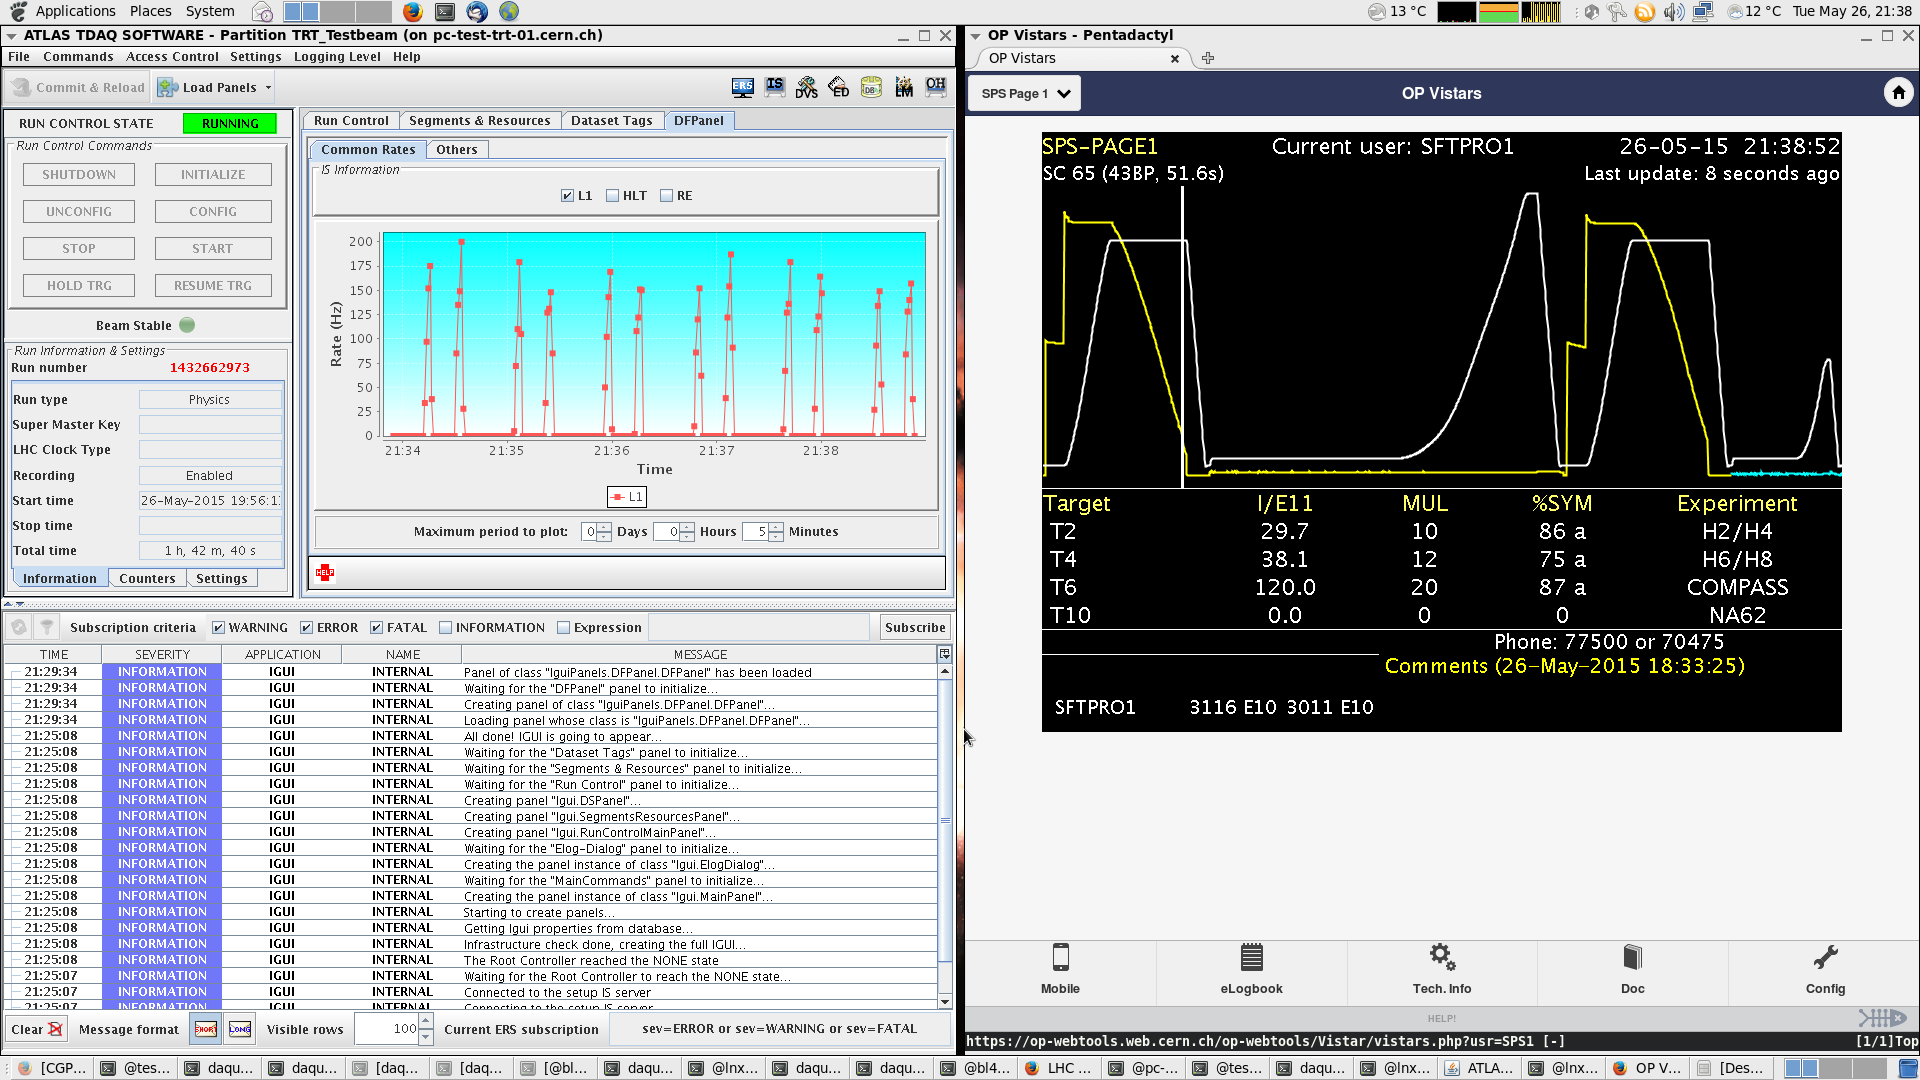
\includegraphics[scale=0.16]{img/TRT_Running}
  \end{figure}
\end{frame}

\section{MRPC}
\begin{frame}{Multigap RPC}
New detector for BL4S 'menu'

High efficiency tracking detector with excellent time resolution ($\sim80\,\text{ps}$)

Technology used in the ALICE ToF detector - uses NINO Front-End cards

Basis of the Extreme Energy Events (EEE) project
\end{frame}

\begin{frame}{MRPC PCBs}
  \begin{figure}
    \centering
    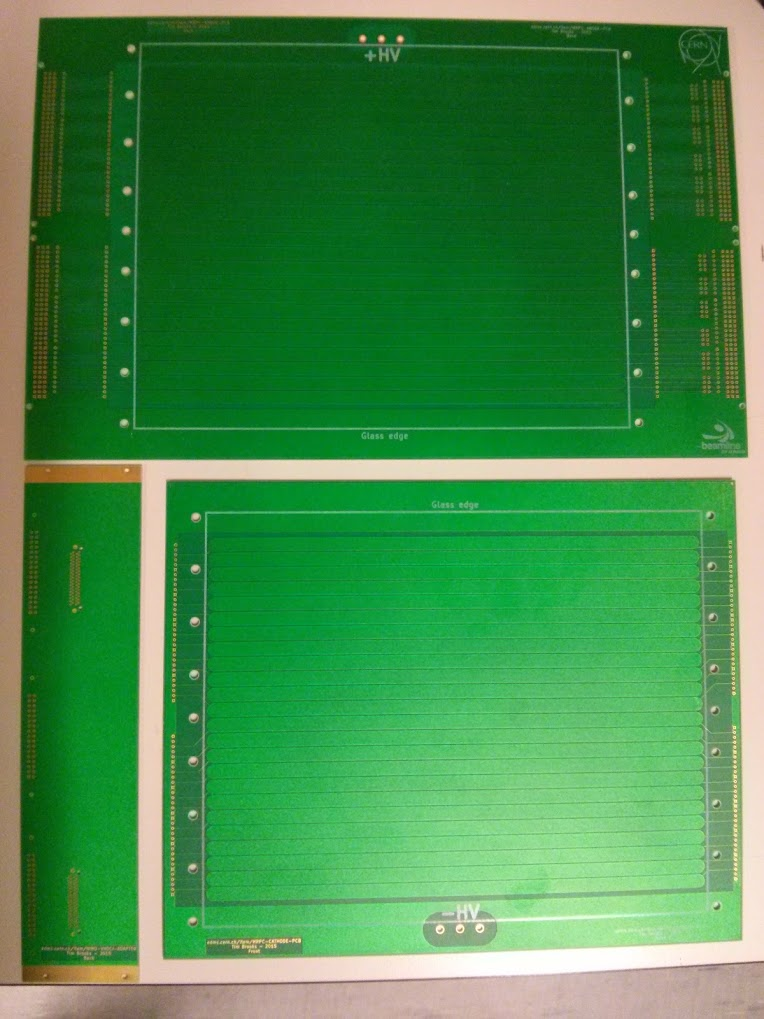
\includegraphics[scale=0.18]{img/outside}
    \,
    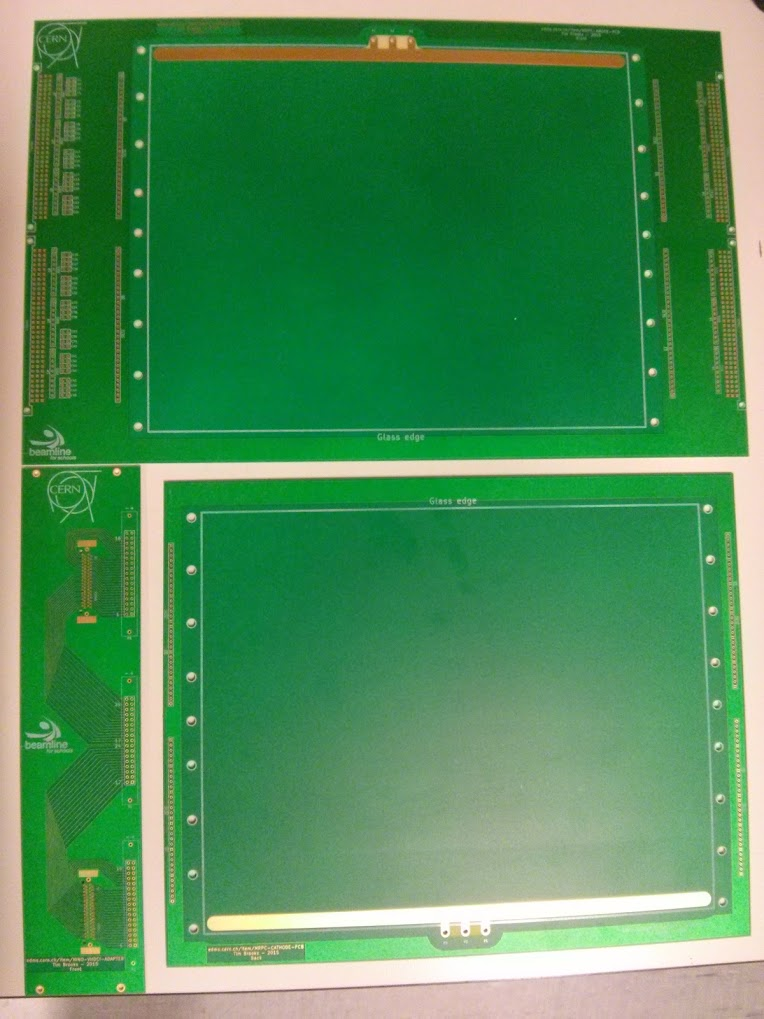
\includegraphics[scale=0.18]{img/inside}
  \end{figure}
\end{frame}

\section{BL4S}

\begin{frame}{Accelerating Africa proposal}
\begin{itemize}
\item Experiment aims to measure synchrotron light emitted by charged particles passing a crystal

\item Team is working with the University of Johannesburg to source/grow crystals

\item Contacts from the University, Prof.~Simon~Connell, Sergio~Ballestrero (Based at CERN)
\begin{itemize}\item Keen to help with experimental design and data analysis:- programming C++, using ROOT
\end{itemize}
\end{itemize}
\end{frame}

\begin{frame}{Experiment set-up}
\begin{itemize}
\item Experiment requires use of Magnetic field to separate charged particles from synchrotron photons

\item Have 6 Scintillators for time reference, trigger

\item Have lead glass calorimeters for photon and deflected beam

\item Have 2 DWCs + one more in T9 Beamline
\end{itemize}
\begin{figure}
  \centering
    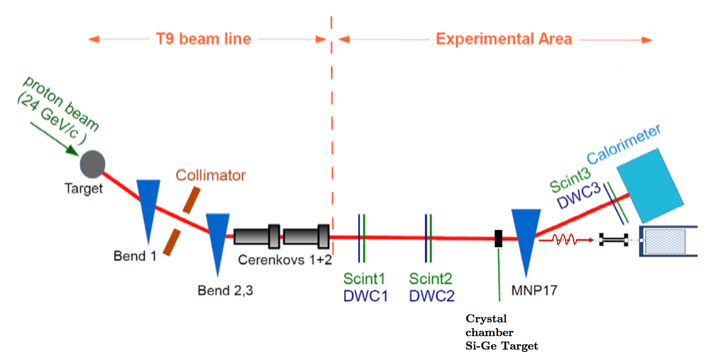
\includegraphics[scale=0.3]{img/AA_layout}
\end{figure}
\end{frame}

\begin{frame}{To Do}
\begin{itemize}
\item Simulations may inform design
\item Need mounting stage to align crystal to beam:-
\begin{itemize}\item UJ has a LabView controlled goniometer \end{itemize}
\item Need to optimise experimental design:-
\begin{itemize}\item Remnant charged beam must be deflected by magnetic field
\item DWC might not be the best tracker for the deflected charged particles\end{itemize}
\item Customise BL4S analysis software for experiment
\end{itemize}
\end{frame}

\end{document}
